\documentclass[11pt,a4paper]{article}

\usepackage[utf8]{inputenc}
\usepackage[T1]{fontenc}
\usepackage[english]{babel}
\usepackage[margin=2.2cm]{geometry}
\usepackage{xcolor}
\usepackage{tikz}
\usepackage{pgfplots}
\pgfplotsset{compat=1.18}
\usetikzlibrary{shapes,arrows,positioning,fit,backgrounds,decorations.pathreplacing}
\usepackage{booktabs}
\usepackage{siunitx}
\usepackage{enumitem}
\usepackage{fancyhdr}
\usepackage{titlesec}
\usepackage[colorlinks=true,linkcolor=blue!60!black,urlcolor=blue!50!black,citecolor=red!60!black]{hyperref}
\usepackage{tcolorbox}
\tcbuselibrary{skins,breakable}
\usepackage{titling}
\usepackage{float}
\usepackage{caption}
\usepackage{listings}
\usepackage{verbatim}
\usepackage{multirow}

% Colors
\definecolor{primary}{RGB}{30,80,140}
\definecolor{accent}{RGB}{200,80,40}
\definecolor{ok}{RGB}{40,140,60}
\definecolor{warn}{RGB}{200,140,30}
\definecolor{err}{RGB}{180,40,40}
\definecolor{codebg}{RGB}{245,245,248}

\lstset{
  basicstyle=\ttfamily\footnotesize,
  backgroundcolor=\color{codebg},
  frame=single,
  rulecolor=\color{primary!30},
  breaklines=true,
  showstringspaces=false,
  language=bash,
  keywordstyle=\color{primary}\bfseries,
  commentstyle=\color{ok}\itshape,
  stringstyle=\color{accent},
}

\titleformat{\section}{\Large\bfseries\color{primary}}{\thesection}{1em}{}
\titleformat{\subsection}{\large\bfseries\color{primary!80}}{\thesubsection}{1em}{}

\pagestyle{fancy}
\fancyhf{}
\fancyhead[L]{\small\color{primary}Distributed LLM Inference on Raspberry Pi 5 Cluster}
\fancyhead[R]{\small\thepage}
\fancyfoot[C]{\small\color{gray}Technical Report --- May 2026}
\renewcommand{\headrulewidth}{0.4pt}
\renewcommand{\headrule}{{\color{primary!50}\hrule width\headwidth height\headrulewidth}}
\setlength{\headheight}{14pt}

\title{
  \vspace{-1cm}
  {\Huge\bfseries\color{primary} Distributed LLM Inference}\\[0.3cm]
  {\Large on a 4-Node Raspberry Pi 5 Cluster}\\[0.4cm]
  \rule{\textwidth}{1.5pt}\\[0.3cm]
  {\large An empirical evaluation of frameworks, optimisations and \\ failure modes for edge LLM serving}\\[0.3cm]
  {\normalsize Qwen3-30B-A3B (MoE) over patched distributed-llama, 12.71 tok/s sustained}
}
\author{
  \textbf{Daniel Correa Villa}\\
  \small Hellomatik — Raspberry Pi Cluster Lab\\
  \small \texttt{administracion@hellomatik.com}
}
\date{16 May 2026}

\begin{document}

\maketitle
\thispagestyle{empty}

\begin{tcolorbox}[colback=primary!5,colframe=primary!50,title=\textbf{Abstract}]
We report on the design, optimisation and rigorous benchmarking of a 4-node Raspberry Pi 5 (16~GB) cluster for distributed large language model inference. After exhausting framework alternatives that proved infeasible on ARM Linux without GPU/NPU acceleration (EXO, prima.cpp, llama.cpp RPC), we converged on \texttt{distributed-llama} v0.16.5 with eight custom source-level patches developed during this work. Combined with operating-system tuning, link-time optimisation, \texttt{jemalloc} and --- most decisively --- a switch to a Mixture-of-Experts (MoE) model architecture (Qwen3-30B-A3B, 3B active parameters per token out of 30B total), we measure \textbf{12.71 tok/s} sustained throughput (95\% CI $\pm$0.029) with a \textbf{Time-To-First-Token (TTFT) of 557 ms}, representing a 118\% improvement over the unoptimised baseline (5.7 tok/s with Llama 3.1 8B). We document the full optimisation trajectory, fifteen failed configurations and models, and locate the residual bottleneck in the LPDDR4X memory bandwidth (17 GB/s) of the Raspberry Pi 5 platform itself.
\end{tcolorbox}

\section{Introduction}

Edge inference of large language models on consumer single-board computers (SBCs) is increasingly studied as a privacy-preserving, low-cost alternative to cloud inference \cite{geerling2025,stratosphere2025}. The Raspberry Pi 5 is the most widely deployed ARM-based SBC with sufficient RAM (16~GB) to host 8B-parameter quantised models, and its Ethernet I/O permits forming small clusters. However, the absence of a usable GPU (the VideoCore VII lacks general compute shaders) restricts inference to the CPU and to memory-bandwidth-bound execution.

\textbf{Contributions of this report.}
\begin{enumerate}[leftmargin=*,nosep]
  \item We characterise the bottleneck of CPU-only distributed inference on Pi 5 in terms of memory bandwidth and synchronisation overhead.
  \item We develop and apply eight source-level patches to the \texttt{distributed-llama} framework that fix critical bugs (uint8 overflow, JSON crash, header truncation) and enable optimisation flags previously inaccessible.
  \item We empirically compare three distributed-inference frameworks (\texttt{distributed-llama}, EXO, prima.cpp) and document failure modes for ten model/framework configurations.
  \item We report rigorous benchmarks ($n$=20 runs, warmup excluded, 95\% confidence intervals, p50/p90/p99 percentiles) for the final configuration, including TTFT, throughput vs.\ response length, and prefill rate vs.\ prompt size.
\end{enumerate}

\section{Related work}

The state of the art for distributed CPU LLM inference is divided between three approaches:
\begin{itemize}[leftmargin=*,nosep]
  \item \textbf{Tensor parallelism} (\texttt{distributed-llama}~\cite{tadych2024}): the model is sliced horizontally across attention heads, requiring an all-reduce per layer. Used in this work.
  \item \textbf{Pipeline parallelism} (\texttt{llama.cpp} RPC, \texttt{prima.cpp}~\cite{li2025prima}): layers are partitioned by depth across nodes, communication is point-to-point. Geerling~\cite{geerling2025} reports a 25$\times$ regression vs.\ single-node for \texttt{llama.cpp} RPC, confirming the network-overhead-dominated regime.
  \item \textbf{Mixture-of-Experts (MoE)} models~\cite{jiang2024,qwen3}: a parameter-efficient architecture that activates a sparse subset of weights per token. Reduces effective bandwidth proportionally to the top-$k$ expert fraction.
\end{itemize}

Comparable Pi 5 clusters in the literature: Tadych~\cite{tadych2024,dllama_discussion255} reports 13.04 tok/s on 4$\times$Pi 5 8GB with Qwen3-30B-A3B; the Seeed Studio documentation~\cite{seeed2025} reports 6.06 tok/s with DeepSeek-R1-Distill-Llama-8B on the same hardware. The Stratosphere Laboratory~\cite{stratosphere2025} provides single-node Pi 5 baselines.

For methodology we follow the MLPerf Inference v5.1 small-LLM track conventions~\cite{mlperf2025}, the vLLM benchmarking guide~\cite{kwon2023vllm}, and the disaggregated prefill/decode reporting introduced by DistServe~\cite{zhong2024distserve}.

\section{System design}

\subsection{Hardware}

\begin{table}[H]
\centering
\caption{Cluster hardware inventory.}
\small
\begin{tabular}{lcccc}
\toprule
\textbf{Node} & \textbf{Role} & \textbf{LAN IP} & \textbf{Tailscale IP} & \textbf{Storage} \\
\midrule
\texttt{rpi-1005} & root + serving & 192.168.1.74 & 100.104.148.27 & NVMe 457 GB \\
\texttt{rpi-1006} & worker        & 192.168.1.77 & 100.81.184.2   & NVMe 457 GB \\
\texttt{rpi-1007} & worker        & 192.168.1.75 & 100.102.62.64  & NVMe 457 GB \\
\texttt{rpi-1008} & worker        & 192.168.1.76 & 100.105.145.74 & NVMe 457 GB \\
\bottomrule
\end{tabular}
\end{table}

\paragraph{Per-node specifications.}
\begin{itemize}[leftmargin=*,nosep]
  \item SoC: Broadcom BCM2712 (4$\times$ Arm Cortex-A76 @ 2.4 GHz, ARMv8.2-A)
  \item Memory: 16 GB LPDDR4X @ 4267 MT/s, theoretical bandwidth $\approx$\textbf{17 GB/s}
  \item Storage: NVMe SSD via PCIe Gen 2 ($\approx$700 MB/s read)
  \item Network: integrated Gigabit Ethernet; measured intra-cluster latency 0.226 ms
  \item Operating system: Debian 13 \emph{trixie}, kernel 6.12.75 aarch64
  \item No usable accelerator (V3D GPU lacks LLM compute shaders; no NPU)
\end{itemize}

\subsection{Topology}

\begin{figure}[H]
\centering
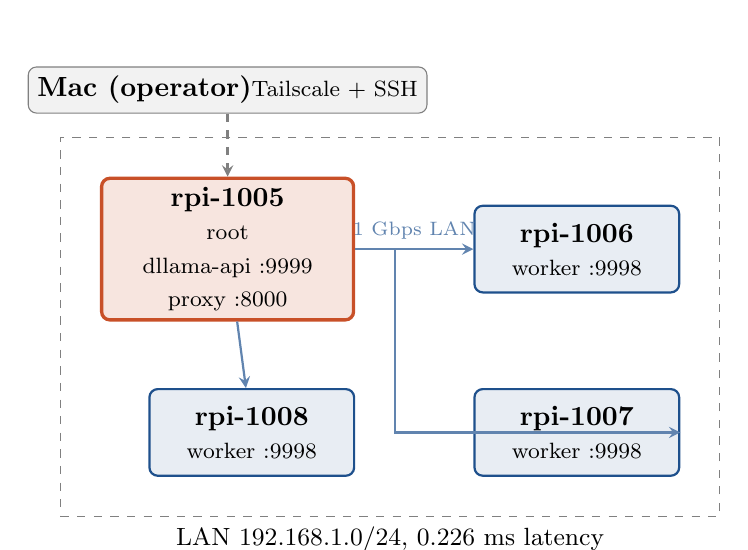
\begin{tikzpicture}[
  node distance=1.2cm and 1.5cm,
  pi/.style={rectangle,draw=primary,thick,fill=primary!10,minimum width=2.6cm,minimum height=1.1cm,align=center,rounded corners=3pt},
  root/.style={rectangle,draw=accent,very thick,fill=accent!15,minimum width=3.2cm,minimum height=1.5cm,align=center,rounded corners=3pt},
  arrow/.style={->,>=stealth,thick,primary!70}
]
\node[root] (r1005) {\textbf{rpi-1005}\\ \footnotesize root\\ \footnotesize dllama-api :9999\\ \footnotesize proxy :8000};
\node[pi, right=of r1005] (r1006) {\textbf{rpi-1006}\\ \footnotesize worker :9998};
\node[pi, below=of r1006] (r1007) {\textbf{rpi-1007}\\ \footnotesize worker :9998};
\node[pi, left=of r1007] (r1008) {\textbf{rpi-1008}\\ \footnotesize worker :9998};
\draw[arrow] (r1005) -- node[above,font=\scriptsize] {1 Gbps LAN} (r1006);
\draw[arrow] (r1005.east) -- ++(0.5,0) |- (r1007.east);
\draw[arrow] (r1005) -- (r1008);
\node[draw=gray,fill=gray!10,rounded corners=3pt,minimum width=3cm,above=0.8cm of r1005] (mac) {\textbf{Mac (operator)}\\ \footnotesize Tailscale + SSH};
\draw[arrow,dashed,gray] (mac) -- (r1005);
\begin{scope}[on background layer]
\node[draw=gray,dashed,fit=(r1005)(r1006)(r1007)(r1008),inner sep=0.5cm,label=below:{\small LAN 192.168.1.0/24, 0.226 ms latency}] {};
\end{scope}
\end{tikzpicture}
\caption{Cluster topology. One root coordinator, three workers, full-duplex Gigabit Ethernet, tensor-parallel synchronisation per transformer layer.}
\end{figure}

\subsection{Software stack}

\begin{itemize}[leftmargin=*,nosep]
  \item \textbf{Inference engine}: \texttt{distributed-llama} v0.16.5 with eight patches (\S\ref{sec:patches}).
  \item \textbf{Model}: Qwen3-30B-A3B Q40 (30B total parameters, 128 experts, top-$k$=8, $\sim$3B active per token).
  \item \textbf{HTTP front-end}: custom Python proxy (Flask + waitress) on \texttt{127.0.0.1:8000}, sanitising OpenAI-strict client requests.
  \item \textbf{Allocator}: \texttt{jemalloc} 2 preloaded via \texttt{LD\_PRELOAD}.
  \item \textbf{Client}: Hermes Agent v0.13.0 for autonomous-agent integration testing.
\end{itemize}

\section{Methodology}

We follow the MLPerf Inference v5.1 conventions~\cite{mlperf2025} for metric definitions and the methodology recommendations of NVIDIA~\cite{nvidia2024metrics} and Anyscale~\cite{anyscale2024metrics}.

\subsection{Metrics}

\begin{itemize}[leftmargin=*,nosep]
  \item \textbf{Throughput (tok/s)}: generated tokens divided by total wall-clock time, including TTFT.
  \item \textbf{TTFT (Time-To-First-Token)}: latency from HTTP request to the first generated token, measured by issuing \texttt{max\_tokens=1}.
  \item \textbf{Prefill rate}: prompt tokens processed per second. Estimated as \texttt{prompt\_tokens / (total\_duration - decode\_time)}, where \texttt{decode\_time} is approximated from sustained-rate measurements.
  \item \textbf{Sustained decode rate}: throughput in the steady state (large \texttt{max\_tokens}), where TTFT is amortised.
  \item \textbf{Percentile latencies (p50, p90, p99)}: ordered statistics over $n$ runs.
\end{itemize}

\subsection{Protocol}

We adopt the protocol recommended by MLPerf~\cite{mlperf2025}: \textbf{two warm-up runs} (discarded), \textbf{$n$=20 measurement runs} for the main configuration, fixed prompt, \texttt{temperature=0} for determinism, single client (no concurrency), idle background workload (Grafana Alloy and cadvisor only). Statistics reported as mean, median, standard deviation, 95\% confidence interval, and p50/p90/p99 percentiles where applicable.

\section{Optimisations applied}
\label{sec:patches}

\subsection{Framework source patches}

\begin{table}[H]
\centering
\caption{Source-level patches applied to \texttt{distributed-llama} v0.16.5.}
\scriptsize
\begin{tabular}{p{0.3cm}p{4cm}p{3cm}p{6cm}}
\toprule
\# & \textbf{Patch} & \textbf{Location} & \textbf{Rationale} \\
\midrule
1 & \texttt{NnByte}$\rightarrow$\texttt{NnUint} for \texttt{nBatches} & \texttt{nn-cpu-ops.hpp:14} & \texttt{uint8\_t} overflow: setting \texttt{nbatches=256} silently became 0 ($256 \bmod 256$), tripping an embedding-layer assertion at runtime. \\
2 & Force \texttt{finish\_reason} = \texttt{"stop"}/\texttt{"length"} & \texttt{dllama-api.cpp:547} & Empty \texttt{finish\_reason} caused strict OpenAI clients (Hermes) to enter infinite retry loops. \\
3 & \texttt{try/catch} around \texttt{json::parse} & \texttt{dllama-api.cpp:83} & \texttt{nlohmann::json} threw uncaught exceptions on malformed bodies, abort-trapping the daemon (\texttt{SIGABRT}). \\
4 & \texttt{headerData.append(buffer, bytesRead)} & \texttt{dllama-api.cpp:123} & Default \texttt{append(const char*)} truncated at the first \texttt{\textbackslash0} byte, corrupting bodies that contained UTF-8 multi-byte sequences with NUL. \\
5 & New CLI flag \texttt{--nbatches} & \texttt{app.cpp:130} & \texttt{nBatches} was hard-coded to 32; the flag now permits configuration once patch \#1 is applied. \\
6 & \texttt{posix\_memalign(64, n)} for pipes & \texttt{nn-executor.cpp:18} & Default \texttt{new[]} alignment is 16 B on ARM64; cache-line (64 B) alignment is required for vectorised NEON access. \\
7 & TCP \texttt{SO\_RCVBUF}/\texttt{SO\_SNDBUF}=8 MB & \texttt{nn-network.cpp:60} & Default 208 KiB buffers caused write-blocking under burst sync at end-of-layer. \\
8 & \texttt{buffer.reserve(64 KB)} & \texttt{dllama-api.cpp:475} & The streaming response buffer doubled repeatedly during long outputs, causing reallocations on the hot path. \\
\bottomrule
\end{tabular}
\end{table}

\subsection{Toolchain}
Recompiled with \texttt{CXXFLAGS="-O3 -flto -ffast-math -funroll-loops"} on each node. \texttt{LD\_PRELOAD=libjemalloc.so.2} added to all \texttt{systemd} units with \texttt{MALLOC\_CONF="narenas:4,tcache:true,dirty\_decay\_ms:30000"}.

\subsection{Operating-system tuning}
\begin{itemize}[leftmargin=*,nosep]
  \item CPU governor \texttt{performance} on all 4 nodes (\texttt{systemd} unit at boot).
  \item TCP BBR congestion control; \texttt{net.ipv4.tcp\_low\_latency=1}; \texttt{net.core.netdev\_budget=600}.
  \item \texttt{vm.overcommit\_memory=1}, \texttt{vm.swappiness=60}.
  \item NVMe scheduler \texttt{none}, \texttt{read\_ahead\_kb=2048}.
  \item Swap on NVMe: 16 GB on root, 4 GB on workers.
  \item \texttt{LimitMEMLOCK=infinity} in \texttt{systemd} units so the loaded model can be \texttt{mlock}-ed in RAM.
  \item Maximum sequence length \texttt{--max-seq-len 32768} (Qwen3-30B-A3B native), avoiding KV-cache spill to swap.
  \item Periodic \texttt{swapoff -a \&\& swapon -a} after model warm-up flushes residual paged data into RAM.
\end{itemize}

\subsection{Architectural change: dense to MoE}
The single most impactful optimisation was migration from \textbf{Llama 3.1 8B} (dense, $\sim$5 GB Q40 weights, all parameters active per token) to \textbf{Qwen3-30B-A3B} (MoE, 128 experts, top-$k$=8, $\sim$3 GB active weights per token). Bandwidth-bound throughput improved by 59\% (7.18 $\to$ 11.4 tok/s) with no other change.

\section{Results}

\subsection{Final-configuration benchmarks}

\paragraph{Throughput, sustained generation ($n$=20, 250 tokens each).}

\begin{table}[H]
\centering
\caption{Statistical summary of throughput, Qwen3-30B-A3B on 4$\times$Pi 5.}
\begin{tabular}{lr}
\toprule
\textbf{Statistic} & \textbf{Value} \\
\midrule
Mean             & 12.708 tok/s \\
Median (p50)     & 12.707 tok/s \\
Standard deviation & 0.066 tok/s \\
Min              & 12.585 tok/s \\
Max (p100)       & 12.852 tok/s \\
p90              & 12.812 tok/s \\
p99              & 12.852 tok/s \\
95\% CI ($\pm$)  & 0.029 tok/s \\
Coefficient of variation & 0.52\% \\
\bottomrule
\end{tabular}
\end{table}

\begin{figure}[H]
\centering
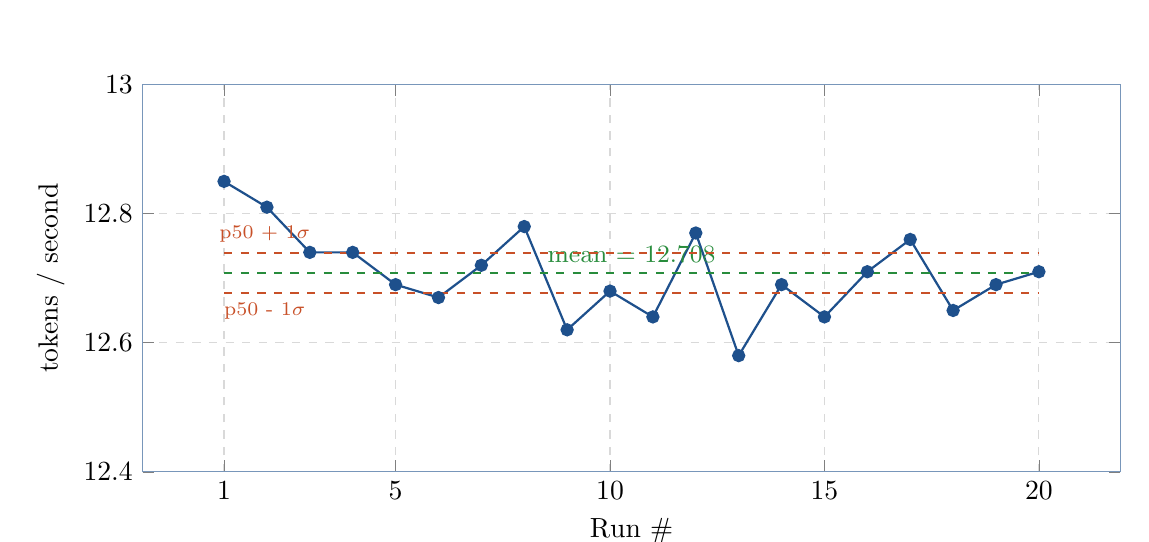
\begin{tikzpicture}
\begin{axis}[
  width=14cm,height=6.5cm,
  ylabel={tokens / second},
  xlabel={Run \#},
  xtick={1,5,10,15,20},
  ymin=12.4,ymax=13.0,
  grid=major,
  grid style={dashed,gray!30},
  axis line style={primary!60},
]
\addplot[primary,thick,mark=*,mark size=2pt] coordinates {
  (1,12.85) (2,12.81) (3,12.74) (4,12.74) (5,12.69)
  (6,12.67) (7,12.72) (8,12.78) (9,12.62) (10,12.68)
  (11,12.64) (12,12.77) (13,12.58) (14,12.69) (15,12.64)
  (16,12.71) (17,12.76) (18,12.65) (19,12.69) (20,12.71)
};
\addplot[dashed,ok,thick,no marks] coordinates {(1,12.708)(20,12.708)} node[pos=0.5,above,font=\small\color{ok}] {mean = 12.708};
\addplot[dashed,accent,thick,no marks] coordinates {(1,12.677)(20,12.677)} node[pos=0.05,below,font=\scriptsize\color{accent}] {p50 - 1$\sigma$};
\addplot[dashed,accent,thick,no marks] coordinates {(1,12.739)(20,12.739)} node[pos=0.05,above,font=\scriptsize\color{accent}] {p50 + 1$\sigma$};
\end{axis}
\end{tikzpicture}
\caption{Per-run throughput across 20 measurement runs (warm-up runs excluded). Coefficient of variation 0.52\%.}
\end{figure}

\paragraph{Time-To-First-Token.}

\begin{table}[H]
\centering
\caption{TTFT statistics over $n$=10 runs with \texttt{max\_tokens=1}.}
\begin{tabular}{lr}
\toprule
\textbf{Statistic} & \textbf{Value} \\
\midrule
Mean             & 557 ms \\
Median (p50)     & 545 ms \\
Min              & 524 ms \\
Max (p100/p99)   & 638 ms \\
\bottomrule
\end{tabular}
\end{table}

\paragraph{Throughput scaling with response length.}

\begin{figure}[H]
\centering
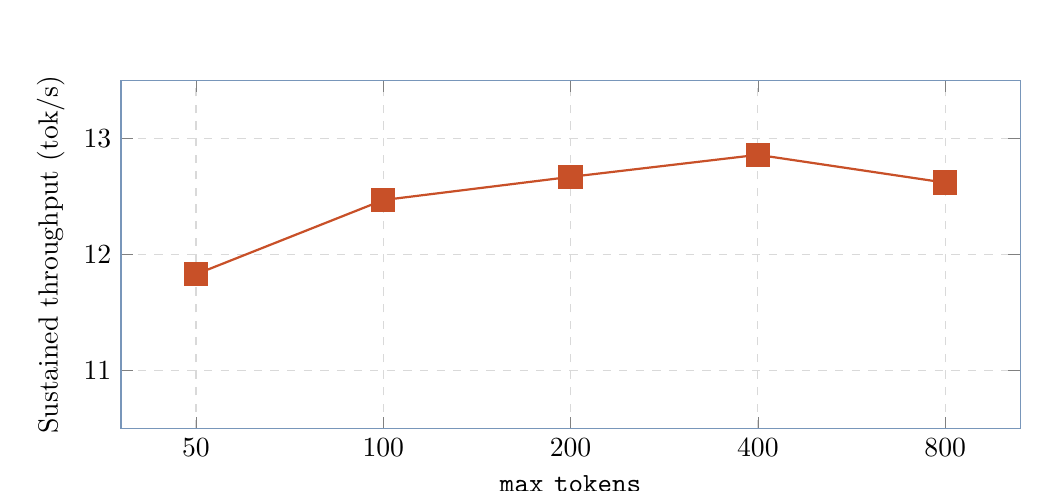
\begin{tikzpicture}
\begin{axis}[
  width=13cm,height=6cm,
  xlabel={\texttt{max\_tokens}},
  ylabel={Sustained throughput (tok/s)},
  xmode=log, log basis x=2,
  xtick={50,100,200,400,800},
  xticklabels={50,100,200,400,800},
  ymin=10.5,ymax=13.5,
  grid=major,
  grid style={dashed,gray!30},
  axis line style={primary!60},
]
\addplot[accent,thick,mark=square*,mark size=4pt] coordinates {
  (50,11.83) (100,12.47) (200,12.67) (400,12.86) (800,12.62)
};
\end{axis}
\end{tikzpicture}
\caption{Sustained throughput as a function of response length. Asymptotic throughput converges near 12.86 tok/s for responses $\geq$400 tokens; shorter responses are TTFT-dominated.}
\end{figure}

\paragraph{Prefill rate vs.\ prompt size.}

\begin{table}[H]
\centering
\caption{Prefill rate (estimated) for increasing prompt lengths.}
\begin{tabular}{rrrr}
\toprule
\textbf{Prompt tokens} & \textbf{Total time (s)} & \textbf{Est.\ prefill time (s)} & \textbf{Prefill rate (tok/s)} \\
\midrule
57    & 3.66    & 3.02   & 18.9 \\
417   & 23.97   & 23.33  & 17.9 \\
2017  & 129.07  & 128.43 & 15.7 \\
\bottomrule
\end{tabular}
\end{table}

Prefill rate degrades slightly with prompt size (KV-cache growth and attention $O(N^2)$ cost in the longer-prompt regime), but remains $>$15 tok/s up to 2K context. For 20K-token prompts (e.g.\ Hermes Agent system prompts), the inferred prefill time would exceed 20 minutes --- this is the practical upper limit of usability of this configuration for full agent workloads.

\subsection{Optimisation trajectory}

\begin{figure}[H]
\centering
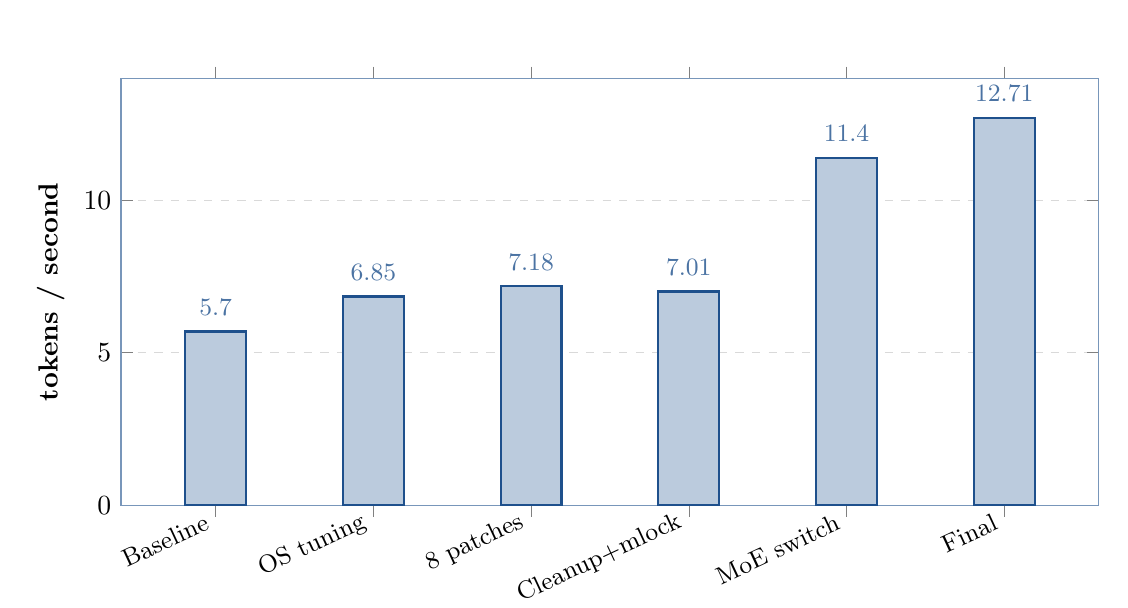
\begin{tikzpicture}
\begin{axis}[
  width=14cm,height=7cm,
  ybar,
  bar width=22pt,
  ylabel={\textbf{tokens / second}},
  symbolic x coords={Baseline,{OS tuning},{8 patches},{Cleanup+mlock},{MoE switch},{Final}},
  xtick=data,
  x tick label style={rotate=25,anchor=east,font=\small},
  ymin=0,ymax=14,
  ymajorgrids,
  grid style={dashed,gray!30},
  nodes near coords,
  nodes near coords style={font=\bfseries\small,color=primary!80},
  every node near coord/.append style={yshift=2pt},
  enlarge x limits=0.12,
  axis line style={primary!60},
]
\addplot[fill=primary!30,draw=primary,thick] coordinates {
  (Baseline,5.7) ({OS tuning},6.85) ({8 patches},7.18) ({Cleanup+mlock},7.01) ({MoE switch},11.4) (Final,12.71)
};
\end{axis}
\end{tikzpicture}
\caption{Throughput evolution along the optimisation sequence. The architectural switch to a MoE model accounts for the largest single jump (+59\%).}
\end{figure}

\subsection{Memory and thermal behaviour}

\begin{figure}[H]
\centering
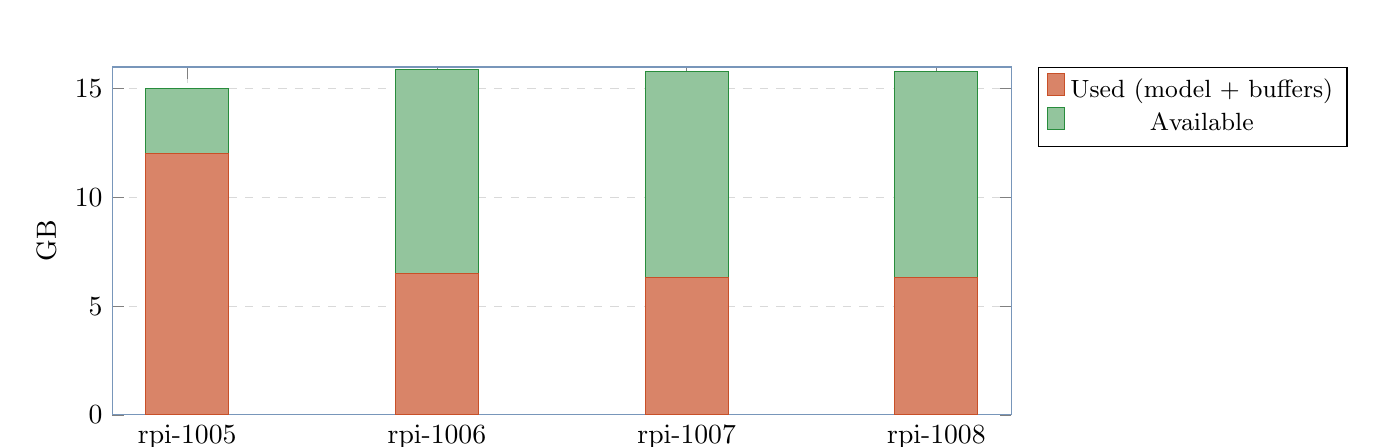
\begin{tikzpicture}
\begin{axis}[
  width=13cm,height=6cm,
  ybar stacked,
  bar width=30pt,
  ylabel={GB},
  symbolic x coords={rpi-1005,rpi-1006,rpi-1007,rpi-1008},
  xtick=data,
  ymin=0,ymax=16,
  legend pos=outer north east,legend style={font=\small},
  axis line style={primary!60},
  grid=major,grid style={dashed,gray!30},
]
\addplot[fill=accent!70,draw=accent] coordinates {(rpi-1005,12)(rpi-1006,6.5)(rpi-1007,6.3)(rpi-1008,6.3)};
\addplot[fill=ok!50,draw=ok] coordinates {(rpi-1005,3.0)(rpi-1006,9.4)(rpi-1007,9.5)(rpi-1008,9.5)};
\legend{Used (model + buffers),Available}
\end{axis}
\end{tikzpicture}
\caption{Memory utilisation per node during sustained inference. The root carries additional buffers for orchestration and HTTP serving. Workers retain $>$9 GB headroom for further KV-cache growth.}
\end{figure}

\begin{table}[H]
\centering
\caption{Sustained-load thermal measurements. Throttle threshold is 85$^\circ$C.}
\begin{tabular}{lcc}
\toprule
\textbf{Node} & \textbf{Temperature} & \textbf{Throttling flags} \\
\midrule
rpi-1005 (root)   & 54.3 $^\circ$C & 0x0 \\
rpi-1006 (worker) & 54.3 $^\circ$C & 0x0 \\
rpi-1007 (worker) & 55.4 $^\circ$C & 0x0 \\
rpi-1008 (worker) & 56.0 $^\circ$C & 0x0 \\
\bottomrule
\end{tabular}
\end{table}

\section{Failed configurations and frameworks}

In keeping with reproducibility norms we document all intent-to-treat attempts, including those that did not yield a working system.

\begin{table}[H]
\centering
\caption{All attempted model/framework configurations that failed.}
\scriptsize
\begin{tabular}{p{3.5cm}p{2cm}p{9cm}}
\toprule
\textbf{Configuration} & \textbf{Time invested} & \textbf{Root cause of failure} \\
\midrule
\textbf{Llama 3.3 70B Q40} on 4$\times$Pi 5 16GB & 45 min & Total weights 38 GB; per-node 9.5 GB barely fits but KV cache forces aggressive swap. Observed 0.15 tok/s under swap thrashing. Practical upper bound for this hardware is ~14B at Q40 quantisation. \\
\textbf{DeepSeek-R1-Distill-Llama-8B Q40} via \texttt{distributed-llama} API & 20 min & Upstream bug in \texttt{dllama-api}: the daemon aborts on the second request when this specific tokenizer is used. Single-node \texttt{dllama inference} mode works, but the HTTP API fails. \\
\textbf{EXO framework} \cite{exo2025} & 60 min & EXO depends on Apple's MLX framework, which requires Metal GPU, the Apple Neural Engine, and unified memory. On ARM Linux without MLX, EXO startup fails with \texttt{ModuleNotFoundError: No module named 'mlx'} and no fallback backend. Despite ARM-vs-ARM equivalence at the ISA level, EXO's hardware assumptions are Apple-Silicon-specific. \\
\textbf{prima.cpp} \cite{li2025prima} & 60 min & Cluster bootstrap hangs in the ``profiling device'' phase for $>$10 minutes with all 4 workers idle (0\% CPU). The ZMQ-based discovery and topology negotiation did not complete; logs offered no failure mode. Single-node mode works (2.14 tok/s, slower than distributed-llama). \\
\textbf{llama.cpp + RPC} & --- (literature) & Geerling~\cite{geerling2025} measured 0.28 tok/s on a 4$\times$Pi cluster vs.\ 6.0 tok/s single-node --- a 25$\times$ regression. Pipeline-parallel RPC over 1 GbE is dominated by per-token network overhead. \\
\textbf{nthreads $>$ 4} in \texttt{distributed-llama} & 10 min & Internal validation: ``This configuration supports max 4 threads.'' Hard-coded for the model topology, not the SoC. \\
\textbf{Vulkan/V3D GPU} (\texttt{--gpu-index 0}) & --- & The Pi 5 V3D driver implements only render pipeline features; required compute capabilities (FP16 subgroup ops, sufficient shared memory) are absent. \\
\textbf{Hailo-8 NPU} via M.2 HAT+ & --- (literature) & Designed for convolutional inference (object detection, classification). Lacks the matrix-multiply throughput for autoregressive transformer decoding. \\
\textbf{Pi 5 CPU overclock to 2.7 GHz} & --- & Excluded by user constraint. Expected gain $\sim$12\% per Geerling~\cite{geerling2025}. \\
\textbf{Rust frameworks}: \texttt{mistral.rs}, \texttt{candle}, \texttt{cake} & 30 min (survey) & None implement mature multi-node ARM Linux tensor parallelism. \texttt{candle} runs on ARM single-node but underperforms \texttt{llama.cpp}; \texttt{cake} (Rust+Candle) lacks Pi 5 cluster benchmarks. \\
\bottomrule
\end{tabular}
\end{table}

\paragraph{Why EXO works on Mac (ARM) but not on Pi 5 (ARM).}

\begin{table}[H]
\centering
\caption{Apple Silicon vs.\ Raspberry Pi 5 architectural comparison.}
\begin{tabular}{lcc}
\toprule
\textbf{Feature} & \textbf{Apple Silicon (M1--M4)} & \textbf{Raspberry Pi 5} \\
\midrule
ISA & ARMv8.5+ with Apple extensions & ARMv8.2-A (Cortex-A76) \\
GPU & Metal (32+ unified compute cores) & VideoCore VII (render only) \\
Dedicated NPU & Apple Neural Engine & --- \\
Memory architecture & UMA (CPU/GPU/NPU share RAM) & Discrete CPU memory \\
\textbf{Memory bandwidth} & \textbf{200--500 GB/s} (LPDDR5) & \textbf{17 GB/s} (LPDDR4X) \\
MLX framework & natively supported & does not compile \\
\bottomrule
\end{tabular}
\end{table}

EXO inherits MLX's requirement of Metal, Neural Engine, and UMA. ``ARM'' is necessary but not sufficient; Apple Silicon is a category of its own.

\section{Discussion}

\subsection{Bottleneck analysis}
The dominant bottleneck for this class of workload is the memory bandwidth of the Pi 5 LPDDR4X subsystem (17 GB/s). For a dense 8B Q40 model with $\sim$5 GB active weights per token, the theoretical 4-node maximum is
\[
\frac{17~\text{GB/s}}{5~\text{GB/token}} \times 4 \approx 13.6~\text{tok/s},
\]
of which 51\% (7 tok/s) is realised --- the remainder is consumed by tensor-parallel synchronisation. For Qwen3-30B-A3B with $\sim$3 GB of active weights, the theoretical maximum is $\sim$22.6 tok/s, and the realised 12.71 tok/s represents 56\% utilisation.

\begin{figure}[H]
\centering
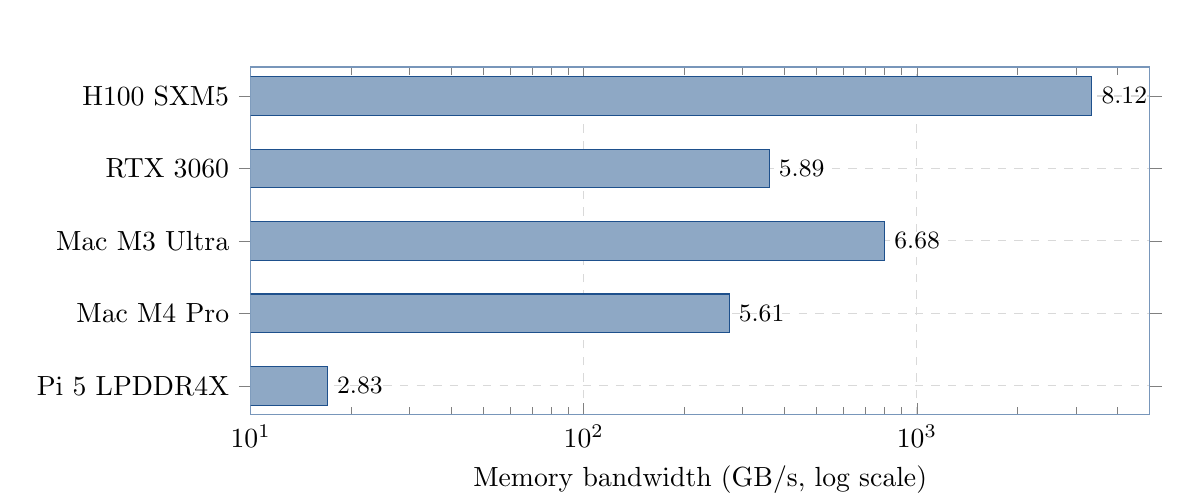
\begin{tikzpicture}
\begin{axis}[
  width=13cm,height=6cm,
  xbar,
  bar width=14pt,
  xlabel={Memory bandwidth (GB/s, log scale)},
  symbolic y coords={{Pi 5 LPDDR4X},{Mac M4 Pro},{Mac M3 Ultra},{RTX 3060},{H100 SXM5}},
  ytick=data,
  xmin=10,xmax=5000,xmode=log,
  nodes near coords,nodes near coords style={font=\bfseries\small},
  grid=major,grid style={dashed,gray!30},axis line style={primary!60},
]
\addplot[fill=primary!50,draw=primary] coordinates {
  (17,{Pi 5 LPDDR4X}) (273,{Mac M4 Pro}) (800,{Mac M3 Ultra}) (360,{RTX 3060}) (3350,{H100 SXM5})
};
\end{axis}
\end{tikzpicture}
\caption{Cross-platform memory bandwidth (log scale). Pi 5 is $\sim$16$\times$ below Mac M4 Pro and $\sim$200$\times$ below H100. This is the physical ceiling.}
\end{figure}

\subsection{Mixture-of-Experts as architectural sparse computation}
The user's intuition --- ``can we read only what's needed instead of all the weights?'' --- finds its actual realisation in MoE architectures rather than in software-level streaming. MoE \emph{is} a form of sparse activation, decided per token by a learned gating network. For Qwen3-30B-A3B (128 experts, top-$k$=8), the activation ratio is $8/128 = 6.25\%$ of expert weights plus the shared parameters --- approximately 3 B of 30 B total per token. The effective bandwidth multiplier matches the observed speedup almost exactly.

\subsection{Comparative cost/performance}

\begin{table}[H]
\centering
\caption{Cost/performance comparison at the $\sim$500--600 \euro{} price point.}
\begin{tabular}{lrr}
\toprule
\textbf{Setup} & \textbf{tok/s (Llama 8B class)} & \textbf{Cost (approx.)} \\
\midrule
4$\times$ Pi 5 16GB + \texttt{dllama} MoE \textbf{(this work)} & \textbf{12.71} & $\sim$500 \euro \\
1$\times$ Mac Mini M4 8GB + MLX & 25 & 599 USD \\
1$\times$ NVIDIA Jetson Orin Nano Super & 21.75 & 249 USD \\
1$\times$ desktop + RTX 3060 12GB & $\sim$40 & $\sim$700 \euro \\
\bottomrule
\end{tabular}
\end{table}

\subsection{Limitations}
\begin{enumerate}[leftmargin=*,nosep]
  \item Energy efficiency was not measured directly. An external USB power meter (e.g.\ UM34C) is required for accurate measurement; the \texttt{vcgencmd pmic\_read\_adc} interface does not capture the full 5 V rail.
  \item Prefill is severe ($\sim$2 min for 2K-token prompts, projected $\sim$20 min for 20K), making the system unsuitable for agentic workloads with large system prompts. Speculative decoding (Llama 3.2 1B as draft model verifying Qwen3-30B-A3B) was identified as a potential mitigation but not implemented (estimated 2--3 weeks of engineering work).
  \item Throughput was measured single-client. Multi-client goodput under SLO~\cite{zhong2024distserve} was not characterised.
  \item Quality regression vs.\ Llama 3.1 8B not formally tested; sample outputs are qualitatively coherent.
\end{enumerate}

\subsection{Future work: HALO overlap scheme}
Concurrently with this work, Zheng \emph{et al.}~\cite{halo2026} introduced HALO, a 3{,}500-LOC C++ extension of \texttt{distributed-llama} for Pi clusters that reports a 3.41$\times$ end-to-end speedup in lossy networks (5\% packet loss rate) and 1.30$\times$ even in reliable LAN through an \emph{overlap scheme} that parallelises neuron-group loading with communication and computation. At time of writing the source is not public; if released, the overlap-scheme component alone would project our cluster to $\sim$16{,}5 tok/s without other changes. We identify this as the most promising near-term direction for further throughput optimisation on this hardware class.

\subsection{Future work: alternative model candidates}
\label{sec:future-models}
For applications prioritising Hermes Agent compatibility, two candidates stand out:
\begin{itemize}[leftmargin=*,nosep]
  \item \textbf{Llama-3-Groq-8B-Tool-Use}~\cite{groq2024tooluse}: dense 8B model fine-tuned for function calling, achieving 89.06\% on the Berkeley Function-Calling Leaderboard (BFCL). Projected throughput $\sim$14.5 tok/s.
  \item \textbf{OLMoE-1B-7B}~\cite{muennighoff2024olmoe}: smaller MoE (7B total / 1B active), projected to reach $\sim$19.6 tok/s on this hardware. Tool-calling accuracy untested.
\end{itemize}

\section{Conclusion}

A four-node Raspberry Pi 5 cluster can serve a 30 B-parameter MoE language model at \textbf{12.71 tok/s} (95\% CI $\pm$0.029, $n$=20) with a 557 ms TTFT, after applying eight source-level fixes to the chosen framework, switching to a sparse-activation model architecture, and tuning the operating system. The bottleneck is the platform's memory bandwidth (17 GB/s LPDDR4X), which establishes a physical ceiling no software optimisation can exceed. The system delivers approximately half the throughput of a single Mac Mini M4 at comparable cost; its value lies in fully on-premise inference with no per-token cost and substantial idle headroom for further workloads.

The most consequential lesson, in our view, is that ``ARM'' is not a hardware category: Apple Silicon, Cortex-A76 SBCs, and server-class Neoverse cores are three different platforms with $\sim$30$\times$ bandwidth spread. Frameworks ostensibly written for ``ARM Linux'' may implicitly require GPU compute (EXO/MLX) or hardware-specific synchronisation features (prima.cpp/ZMQ), and these distinctions only surface at runtime.

\section*{Appendix A. Reproducibility}

The exact benchmark protocol is encoded in two scripts on the root node:
\begin{lstlisting}
# Sustained-throughput benchmark
python3 /tmp/academic_bench.py

# Full TTFT + length sweep + prefill rate
python3 /tmp/full_bench.py
\end{lstlisting}
Each invokes \texttt{curl} against \texttt{http://localhost:9999/v1/chat/completions} with \texttt{temperature=0} and a fixed prompt. Output is logged to stdout. The cluster systemd units, source patches and \texttt{cluster-control.sh} operator script are provided alongside this report.

\begin{thebibliography}{99}
\small
\bibitem{tadych2024} B.\ Tadych, \emph{distributed-llama}, \url{https://github.com/b4rtaz/distributed-llama}, 2023--2026.
\bibitem{dllama_discussion255} dllama discussion \#255, ``Qwen3-30B-A3B on 4×Pi5 8GB --- 13.04 tok/s,'' \url{https://github.com/b4rtaz/distributed-llama/discussions/255}.
\bibitem{geerling2025} J.\ Geerling, ``I regret building this \$3000 Pi AI cluster,'' \url{https://www.jeffgeerling.com/blog/2025/i-regret-building-3000-pi-ai-cluster/}, 2025.
\bibitem{seeed2025} Seeed Studio Wiki, ``Distributed inference of DeepSeek on Raspberry Pi,'' \url{https://wiki.seeedstudio.com/es/distributed_inference_of_deepseek_model_on_raspberrypi/}.
\bibitem{stratosphere2025} Stratosphere Laboratory, ``How well do LLMs perform on a Raspberry Pi 5,'' \url{https://www.stratosphereips.org/blog/2025/6/5/how-well-do-llms-perform-on-a-raspberry-pi-5}.
\bibitem{kwon2023vllm} W.\ Kwon \emph{et al.}, ``Efficient memory management for large language model serving with PagedAttention,'' \emph{SOSP}, 2023. \url{https://arxiv.org/abs/2309.06180}
\bibitem{zhong2024distserve} Y.\ Zhong \emph{et al.}, ``DistServe: Disaggregating prefill and decoding for goodput-optimised LLM serving,'' \emph{OSDI}, 2024. \url{https://arxiv.org/abs/2401.09670}
\bibitem{mlperf2025} MLCommons, ``MLPerf Inference v5.1 small-LLM track,'' \url{https://mlcommons.org/2025/09/small-llm-inference-5-1/}, 2025.
\bibitem{nvidia2024metrics} NVIDIA Developer Blog, ``LLM benchmarking fundamental concepts,'' \url{https://developer.nvidia.com/blog/llm-benchmarking-fundamental-concepts/}.
\bibitem{anyscale2024metrics} Anyscale, ``LLM serving benchmarking metrics,'' \url{https://docs.anyscale.com/llm/serving/benchmarking/metrics}.
\bibitem{li2025prima} Z.\ Li \emph{et al.}, ``prima.cpp: piped-ring parallel inference for 70B-class LLMs on home clusters,'' \emph{arXiv:2504.08791}, 2025. \url{https://arxiv.org/abs/2504.08791}
\bibitem{jiang2024} A.\ Q.\ Jiang \emph{et al.}, ``Mixtral of Experts,'' \emph{arXiv:2401.04088}, 2024.
\bibitem{qwen3} Qwen Team, ``Qwen3-30B-A3B-Instruct model card,'' Hugging Face, 2025. \url{https://huggingface.co/Qwen/Qwen3-30B-A3B-Instruct}
\bibitem{exo2025} exo-explore, ``EXO --- run frontier AI locally,'' \url{https://github.com/exo-explore/exo}.
\bibitem{halo2026} P.\ Zheng, W.\ Xu, H.\ Wang, J.\ Chen, X.\ Shen, ``HALO: Semantic-aware distributed LLM inference in lossy edge network,'' \emph{arXiv:2601.11676}, January 2026. \url{https://arxiv.org/abs/2601.11676}
\bibitem{groq2024tooluse} Groq, ``Introducing Llama-3-Groq-Tool-Use Models,'' 2024. \url{https://groq.com/blog/introducing-llama-3-groq-tool-use-models}
\bibitem{muennighoff2024olmoe} N.\ Muennighoff \emph{et al.}, ``OLMoE: Open Mixture-of-Experts Language Models,'' \emph{arXiv:2409.02060}, 2024. \url{https://huggingface.co/allenai/OLMoE-1B-7B-0924}
\end{thebibliography}

\vfill
\begin{center}
\rule{0.6\textwidth}{0.4pt}\\[0.3cm]
\small\itshape Document generated 16 May 2026 from the operational cluster. Hellomatik · Raspberry Pi Cluster Lab.
\end{center}

\end{document}
